\documentclass[11pt, a4paper]{article}
\usepackage{graphicx}
\usepackage{amsmath}
\usepackage{listings}

\title{Assignment 4}
\author{G Ch V Sairam , EE19B081}
\date{10-03-2021}

\begin{document}		
\maketitle
\section*{Introduction}
The Fourier series of any function which is periodic with period 2pi is calculated as follows: 
\begin{equation*}
	f(x)=a_0+ \sum_{n=1}^{\infty} {a_n cos(nx)+b_n sin(nx)}
\end{equation*}
where $a_n$ , $b_n$ are called the fourier series coefficients.
\begin{itemize}
  	\item $a_0$= 1/2$\pi$ $ \int_{0}^{2pi} f(x) \,dx $
  	\item $a_n$= 1/2$\pi$ $ \int_{0}^{2pi} f(x)cos(nx) \,dx $
  	\item $b_n$= 1/2$\pi$ $ \int_{0}^{2pi} f(x)sin(nx) \,dx $
\end{itemize}


\section*{Assignment problems}
\subsection*{Question 1}
The functions are defined in the following way:
\lstinputlisting[language=Python, firstline=10, lastline=15]{EE19B081_assign4.py}

Here , the functions np.exp() and np.cos() are used instaed of math.exp() and math.cos() because the former can accept vector inputs and generate vector ouputs but the latter cannot.

cos(cos(x)) is periodic but $e^x$ is not periodic. But the fourier series generates only periodic functions. So , I expect that the functons cos(cos(x)) and $e^y$ will be generated where y is the remainder obtained when x is divided by $2\pi$.

We can find the periodic extension of $e^x$ as mentioned in the below code line:
\lstinputlisting[language=Python, firstline=21, lastline=21]{EE19B081_assign4.py}

\begin{figure}[!tbh]
\centering
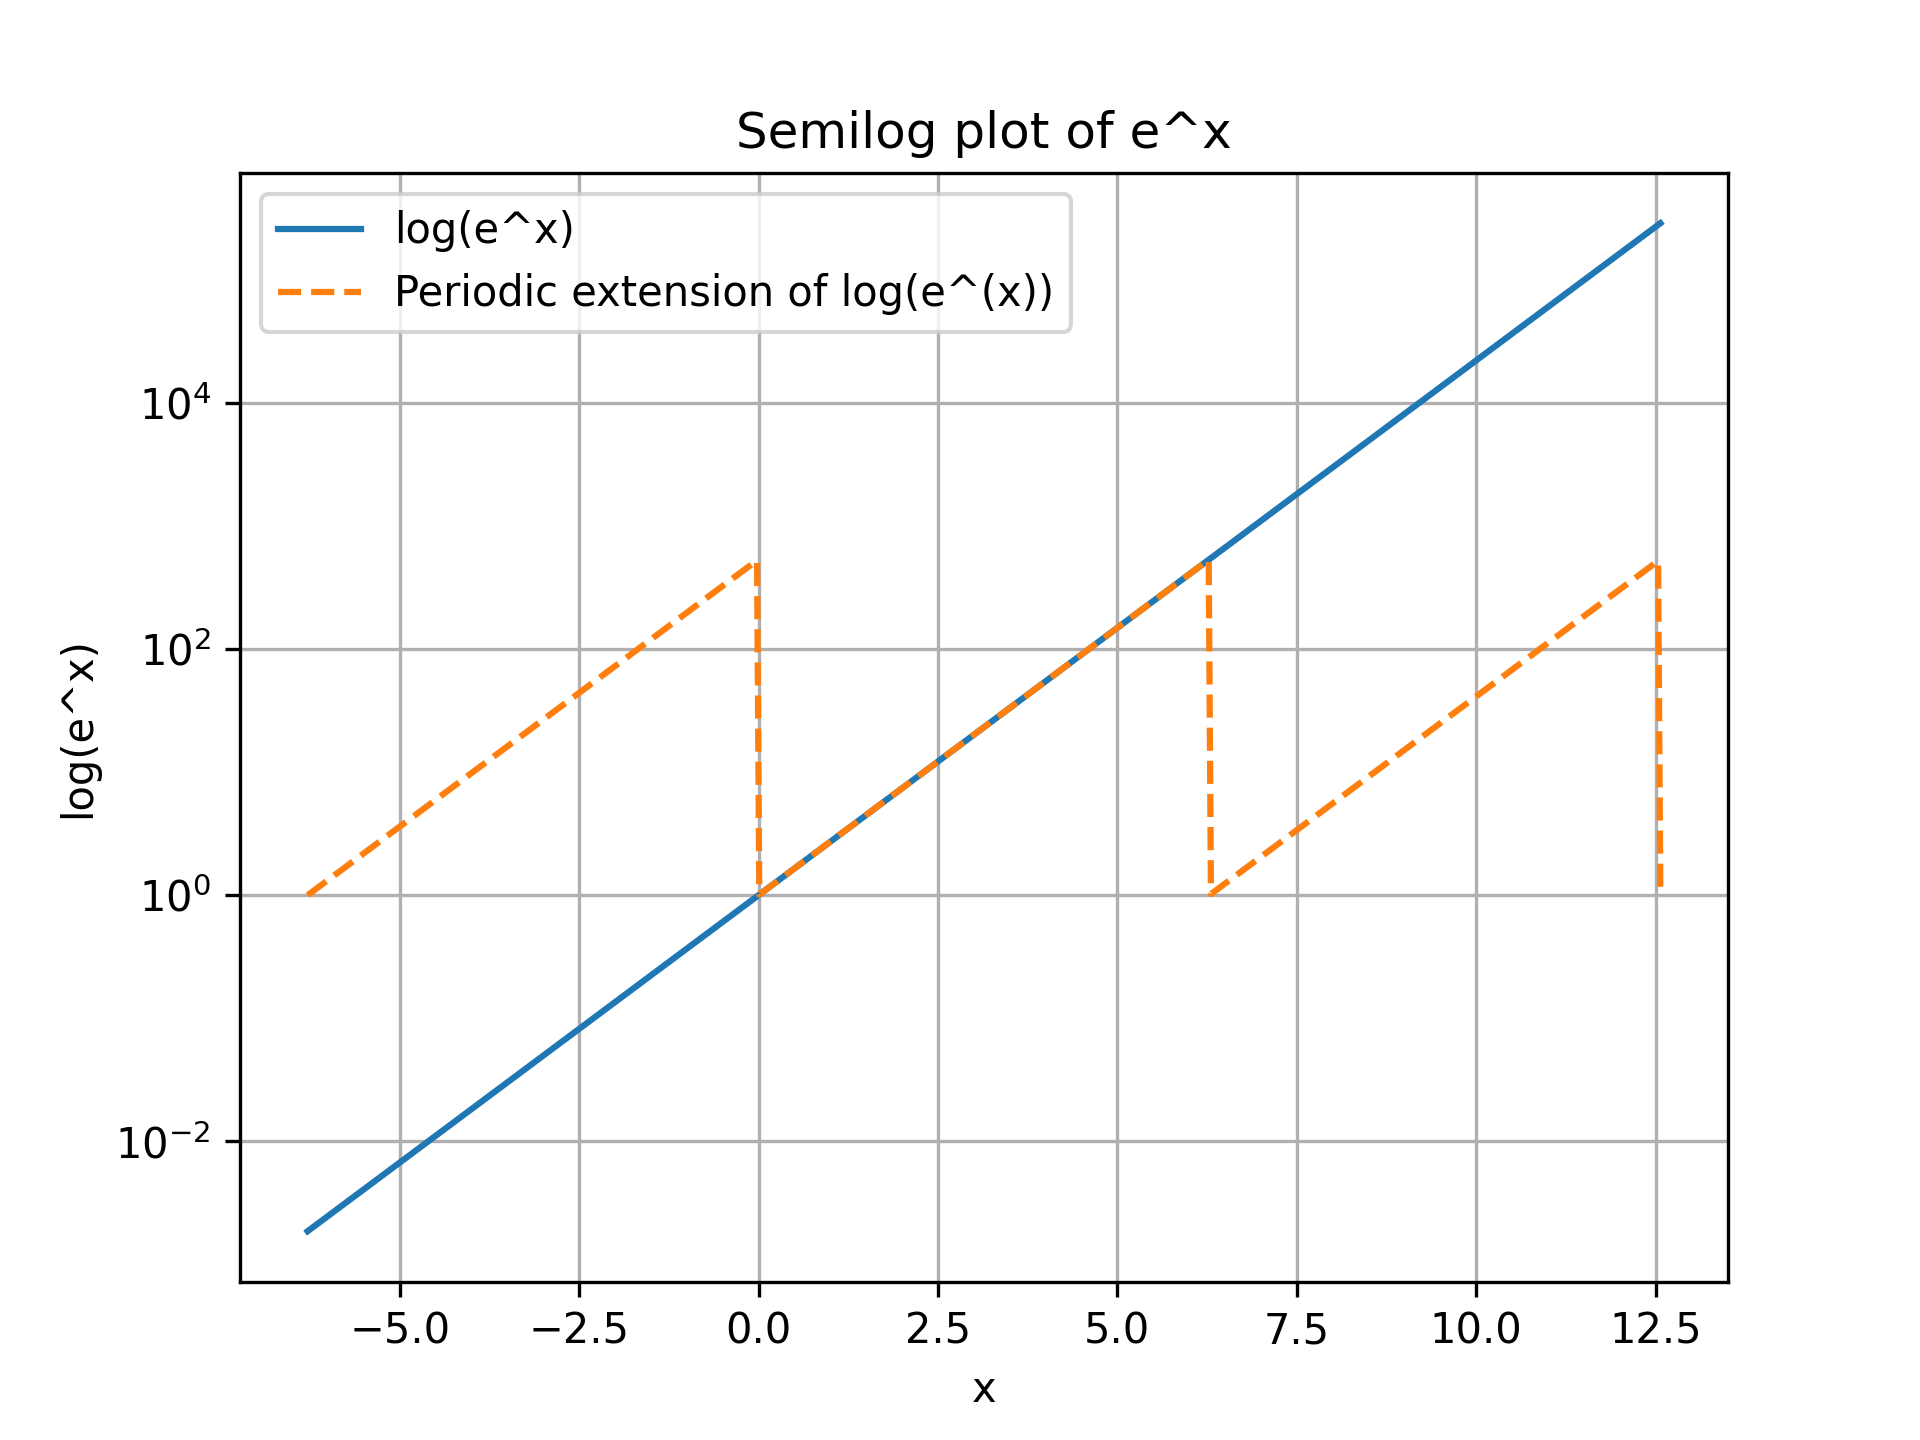
\includegraphics[scale=0.6]{assn4_plot1.png}
\caption{Figure 1}
\label{fig:plot1}
\end{figure} 

\begin{figure}[!tbh]
\centering
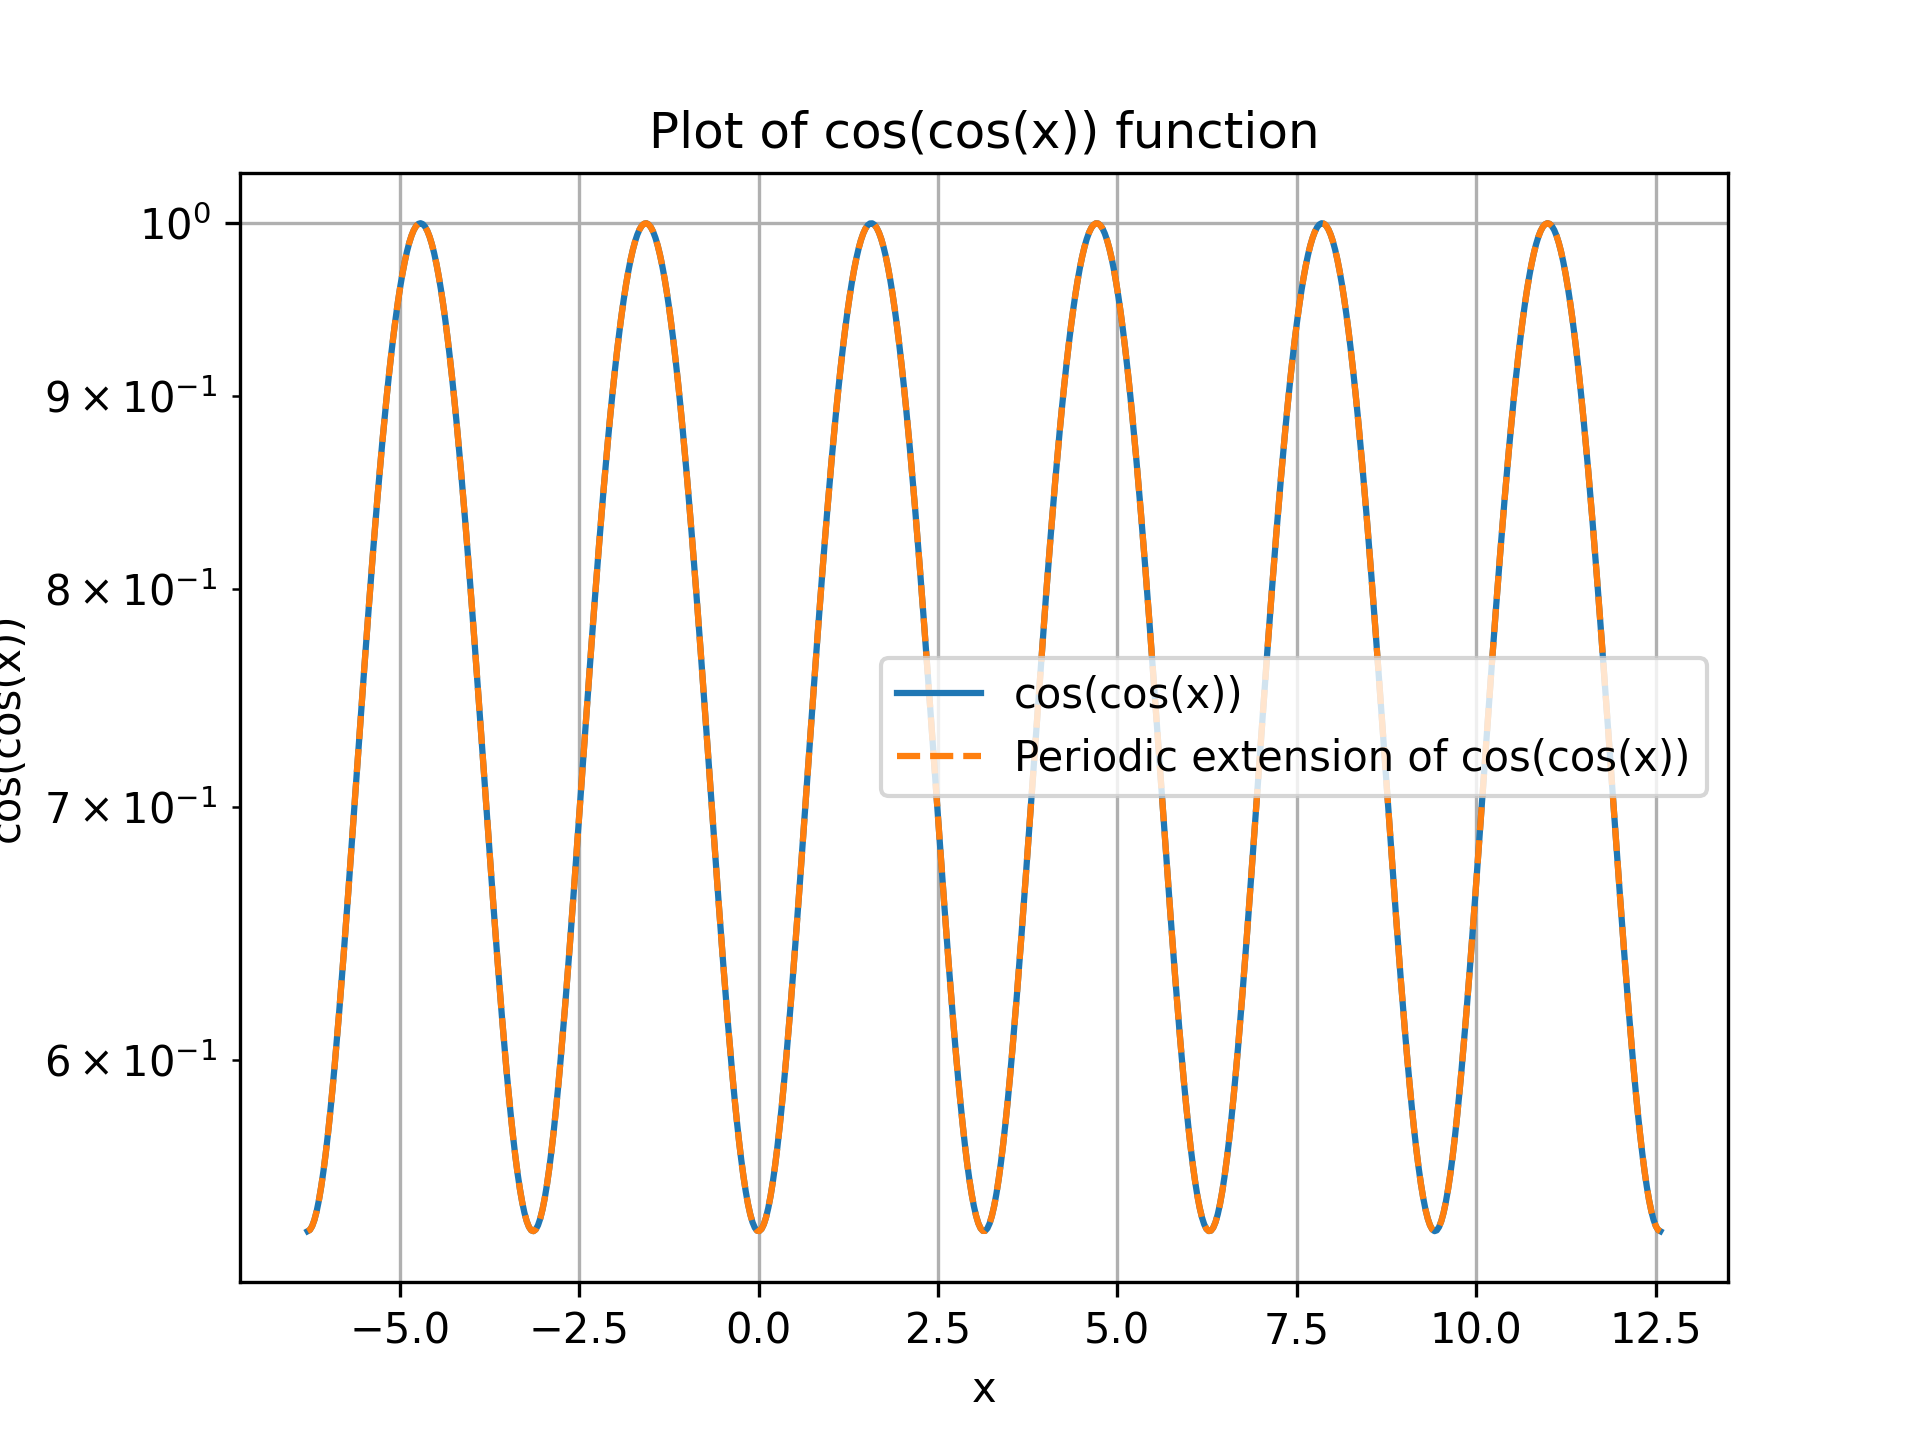
\includegraphics[scale=0.6]{assn4_plot2.png}
\caption{Figure 2}
\label{fig:plot2}
\end{figure} 

\subsection*{Question 2}
The first 51 fourier coefficients of both the functions are calculated using quad function from the scipy.integrate module.
\lstinputlisting[language=Python, firstline=42, lastline=68]{EE19B081_assign4.py}

\subsection*{Question 3}

a)As we know , cos(cos(x)) is an even function. $b_n$ are the coefficients of the term sin(kx), which is an odd function. cos(cos(x)) has no odd part , so for the second case all $b_n$ are nearly zero.

b)For $e^x$ , the higher frequencies also have significant components whereas for cos(cos(x)) the frequency is 1/$\pi$ and hence it doesn't have significant components from the higher frequencies..This is the reason why the coefficients in the first case do not decay as quickly as the coefficients for the second case.

c)For exp(x) , the fourier coefficients,
$a_n$ are proportional to $1/(1+n^2)$,
$b_n$ are proportional to $n/(1+n^2)$.

For large n , $a_n$=$1/n^2$ and $b_n$=$1/n$ .
Therefore , $log(a_n)=$-2log(n) and $log(b_n)=$-log(n).
This is the reason for the linearity of loglog plot in figure 4.
For cos(cos(x)),
the fourier coefficients vary exponentially with n and hence the semilog plot of figure 5 looks linear.

\begin{figure}[!tbh]
\centering
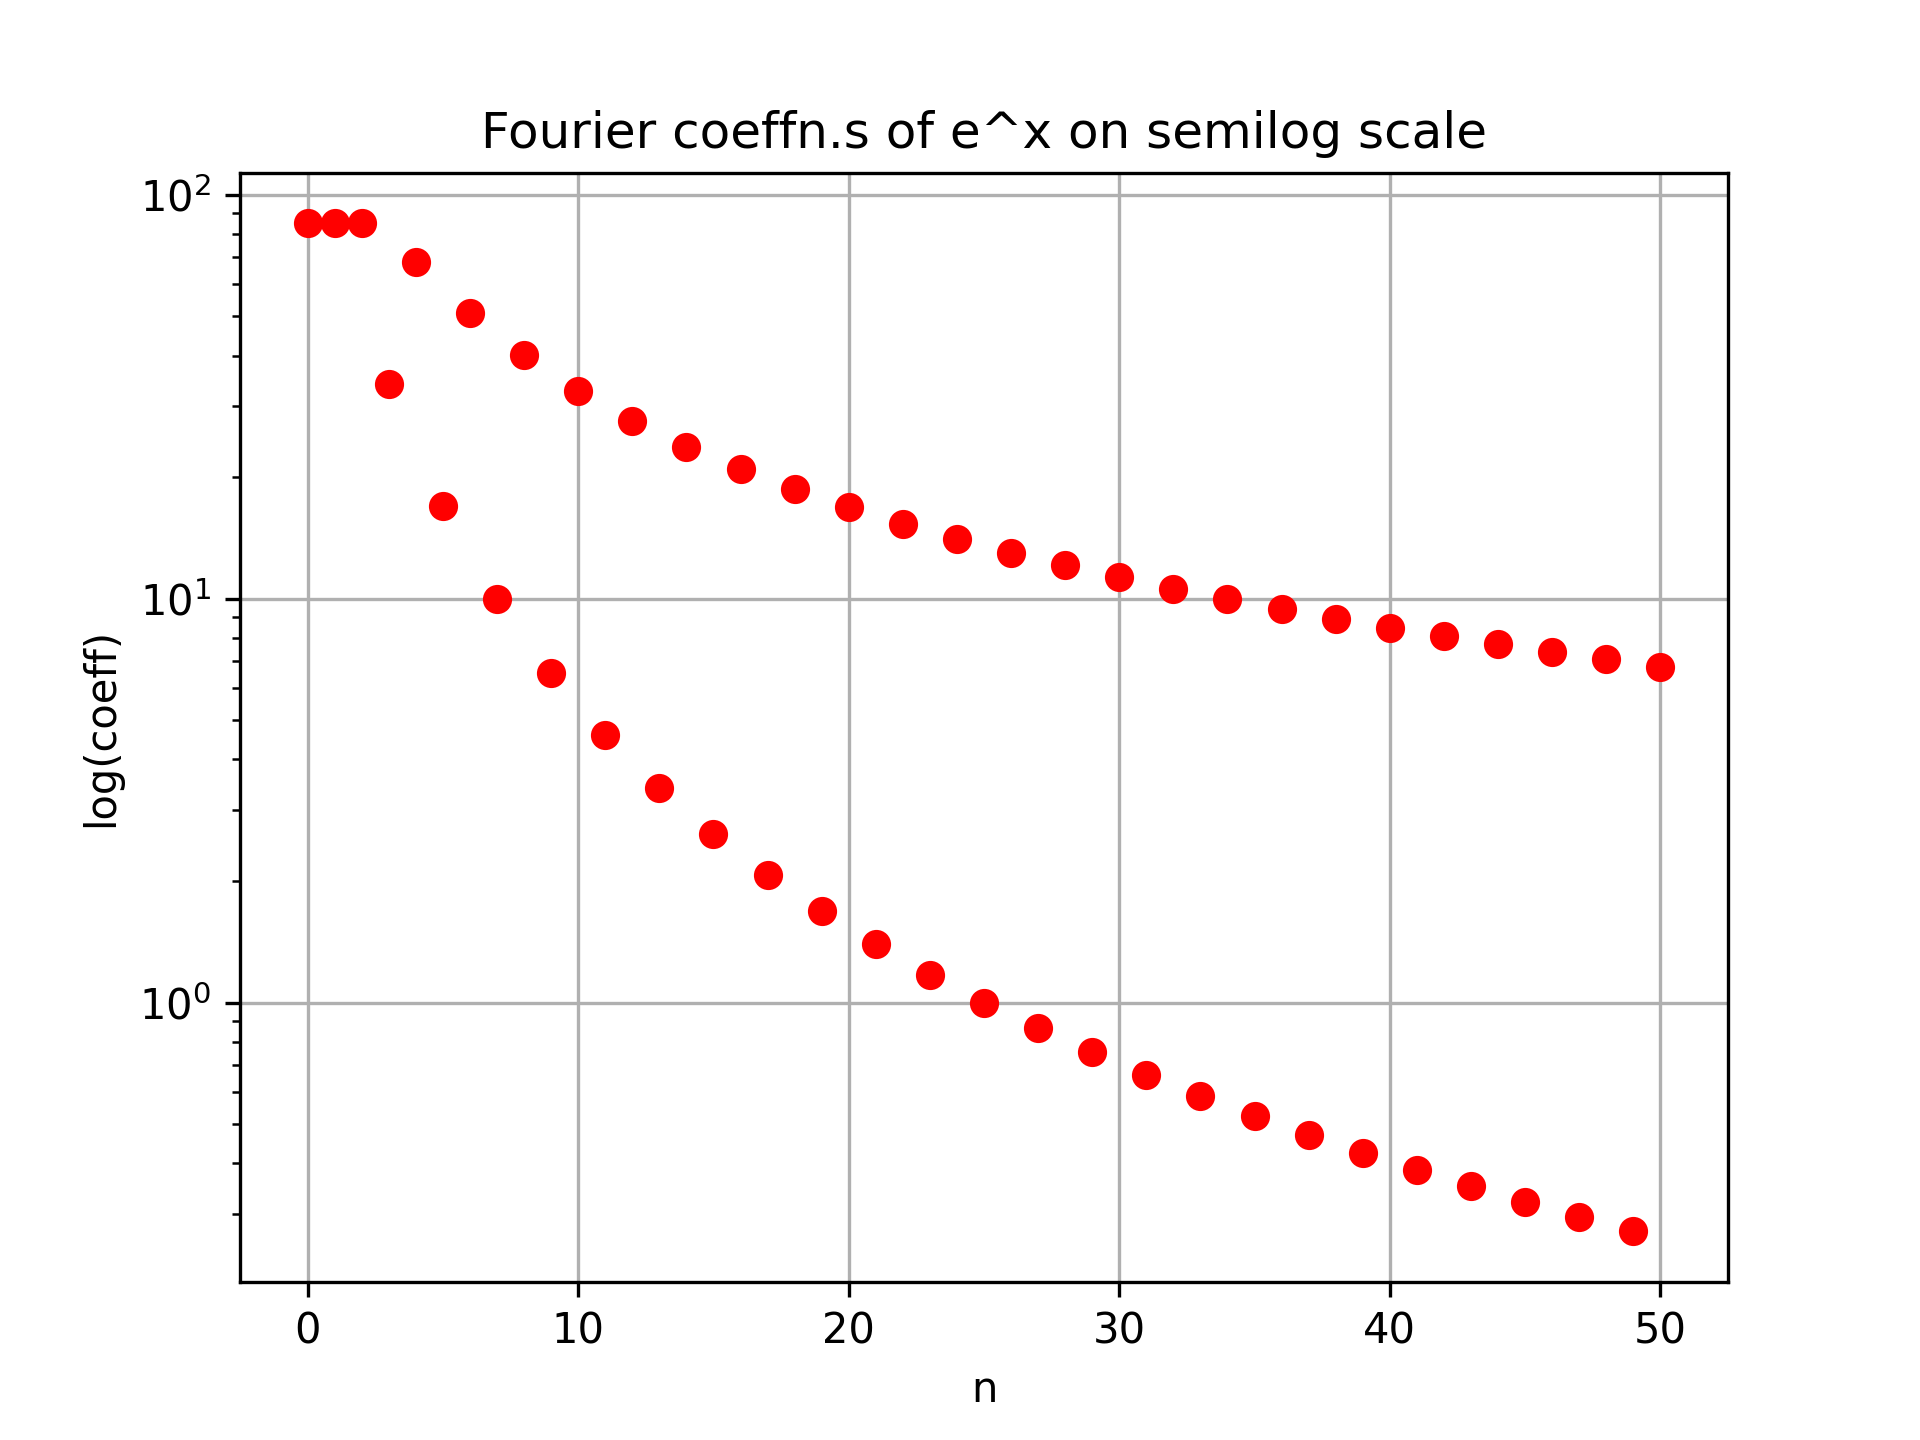
\includegraphics[scale=0.6]{assn4_plot3.png}
\caption{Figure 3}
\label{fig:plot3}
\end{figure} 

\begin{figure}[!tbh]
\centering
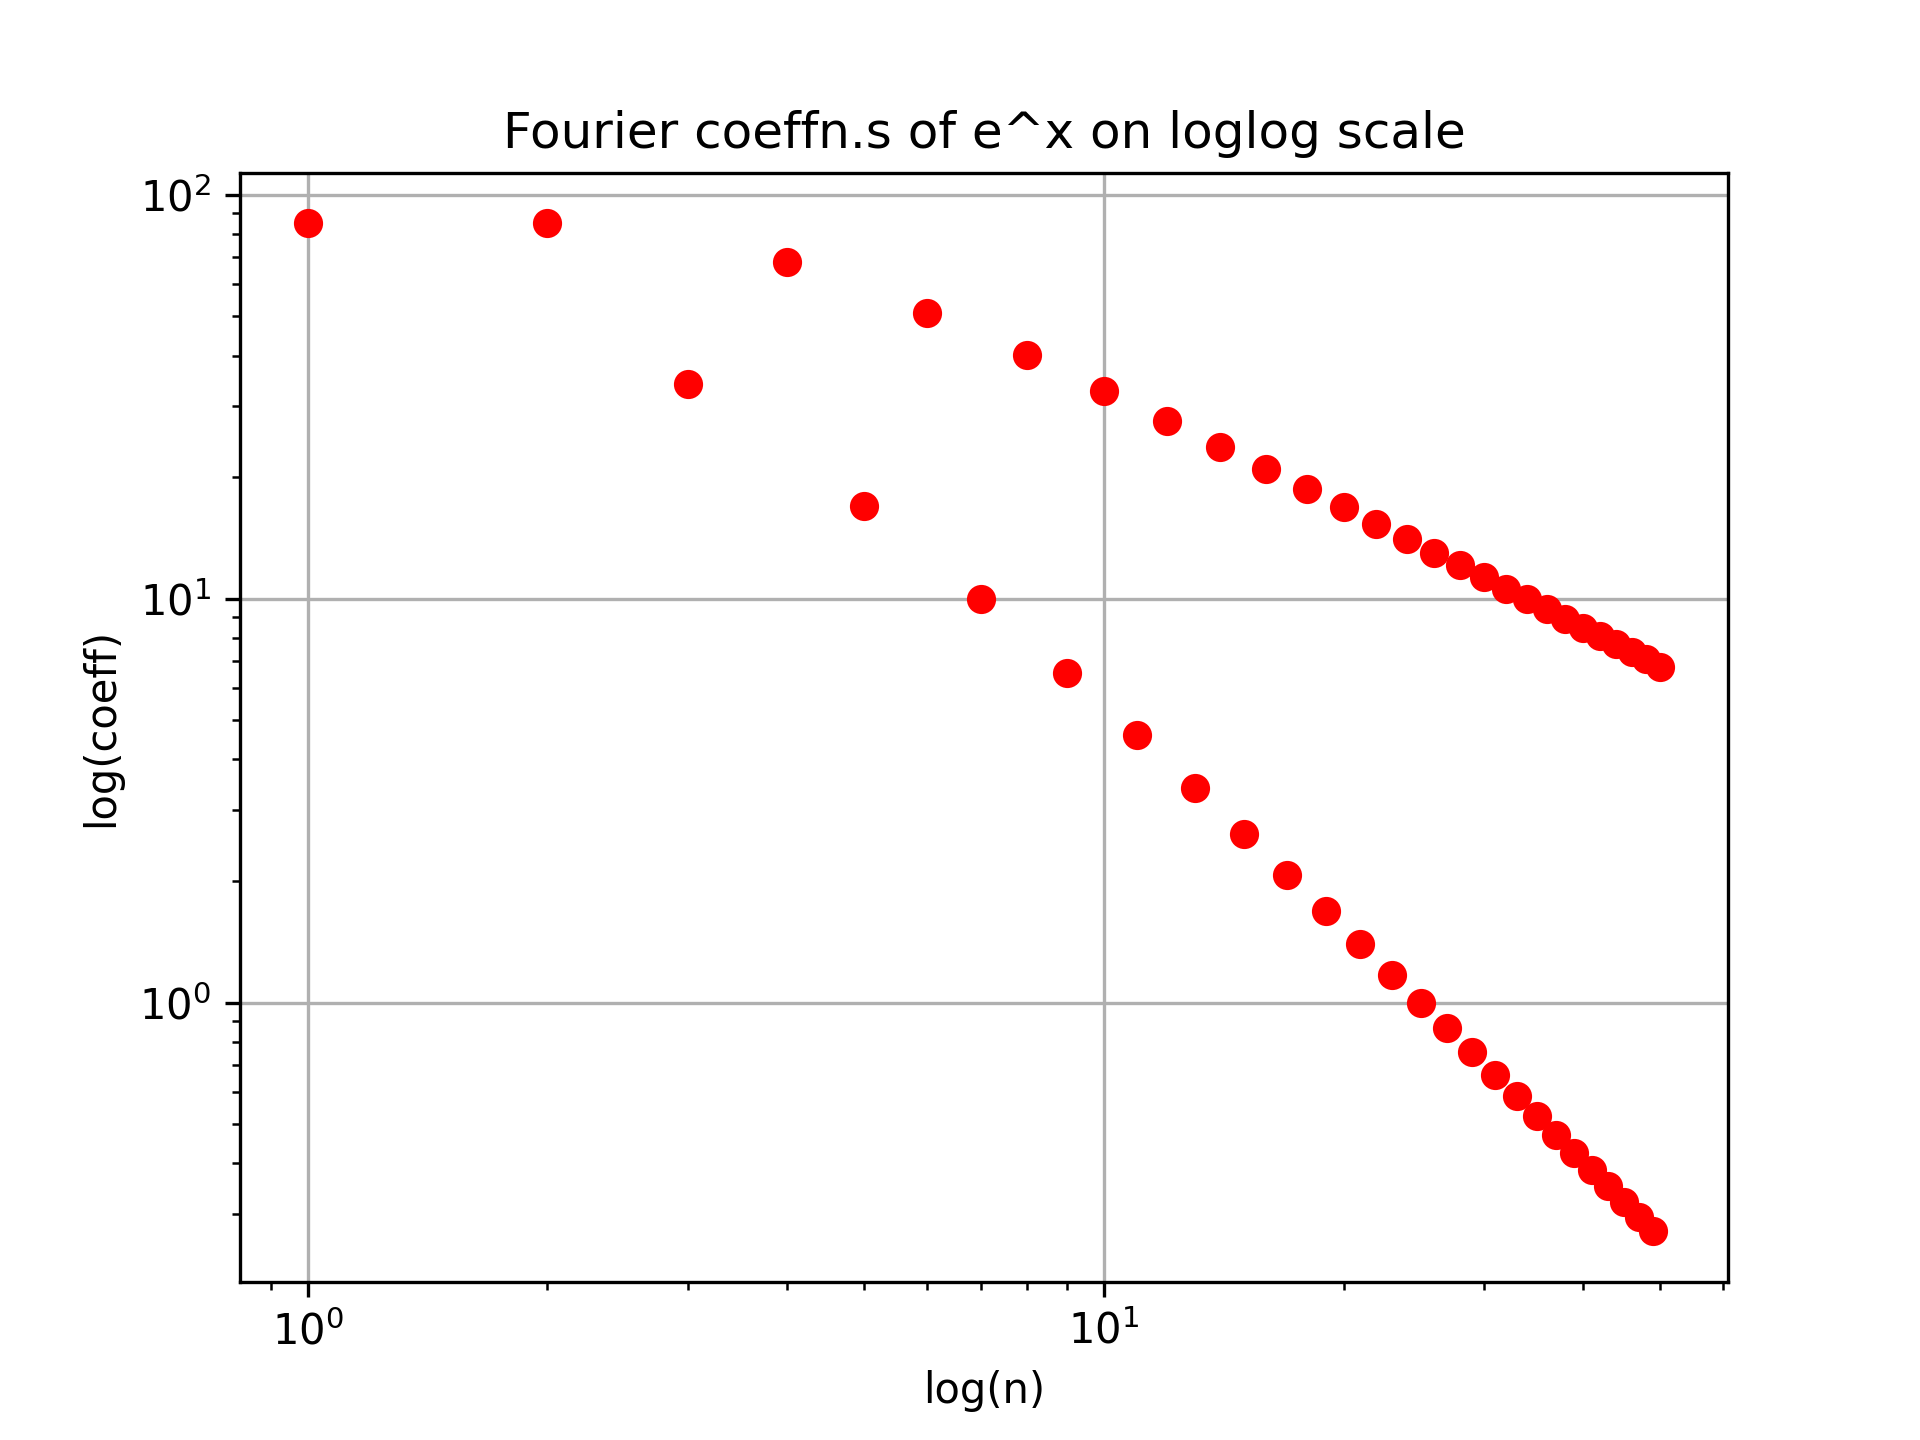
\includegraphics[scale=0.6]{assn4_plot4.png}
\caption{Figure 4}
\label{fig:plot4}
\end{figure} 

\begin{figure}[!tbh]
\centering
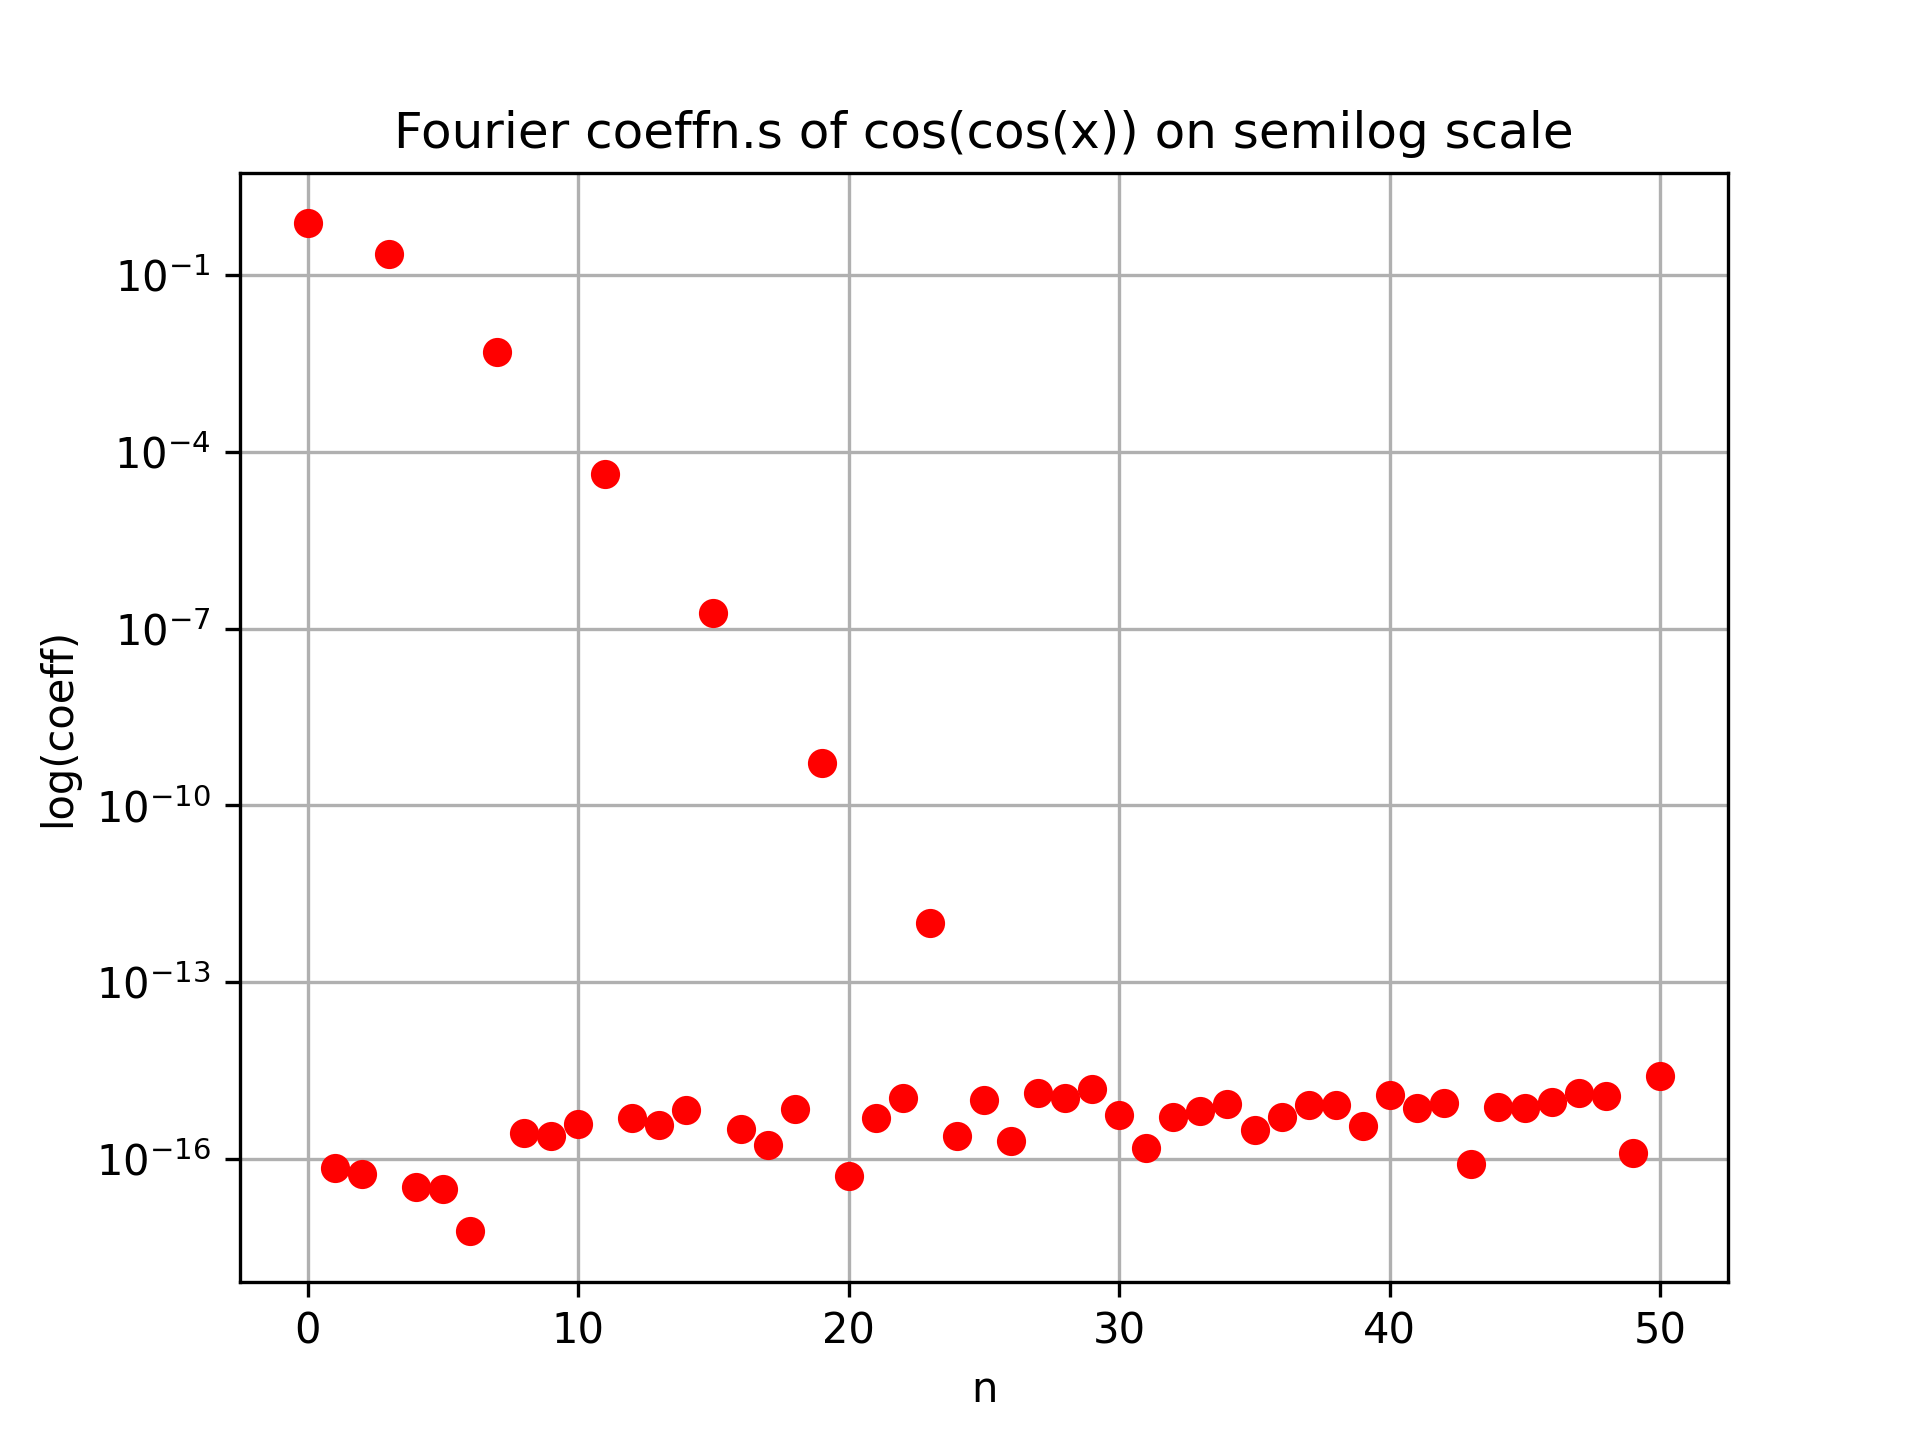
\includegraphics[scale=0.6]{assn4_plot5.png}
\caption{Figure 5}
\label{fig:plot5}
\end{figure} 

\begin{figure}[!tbh]
\centering
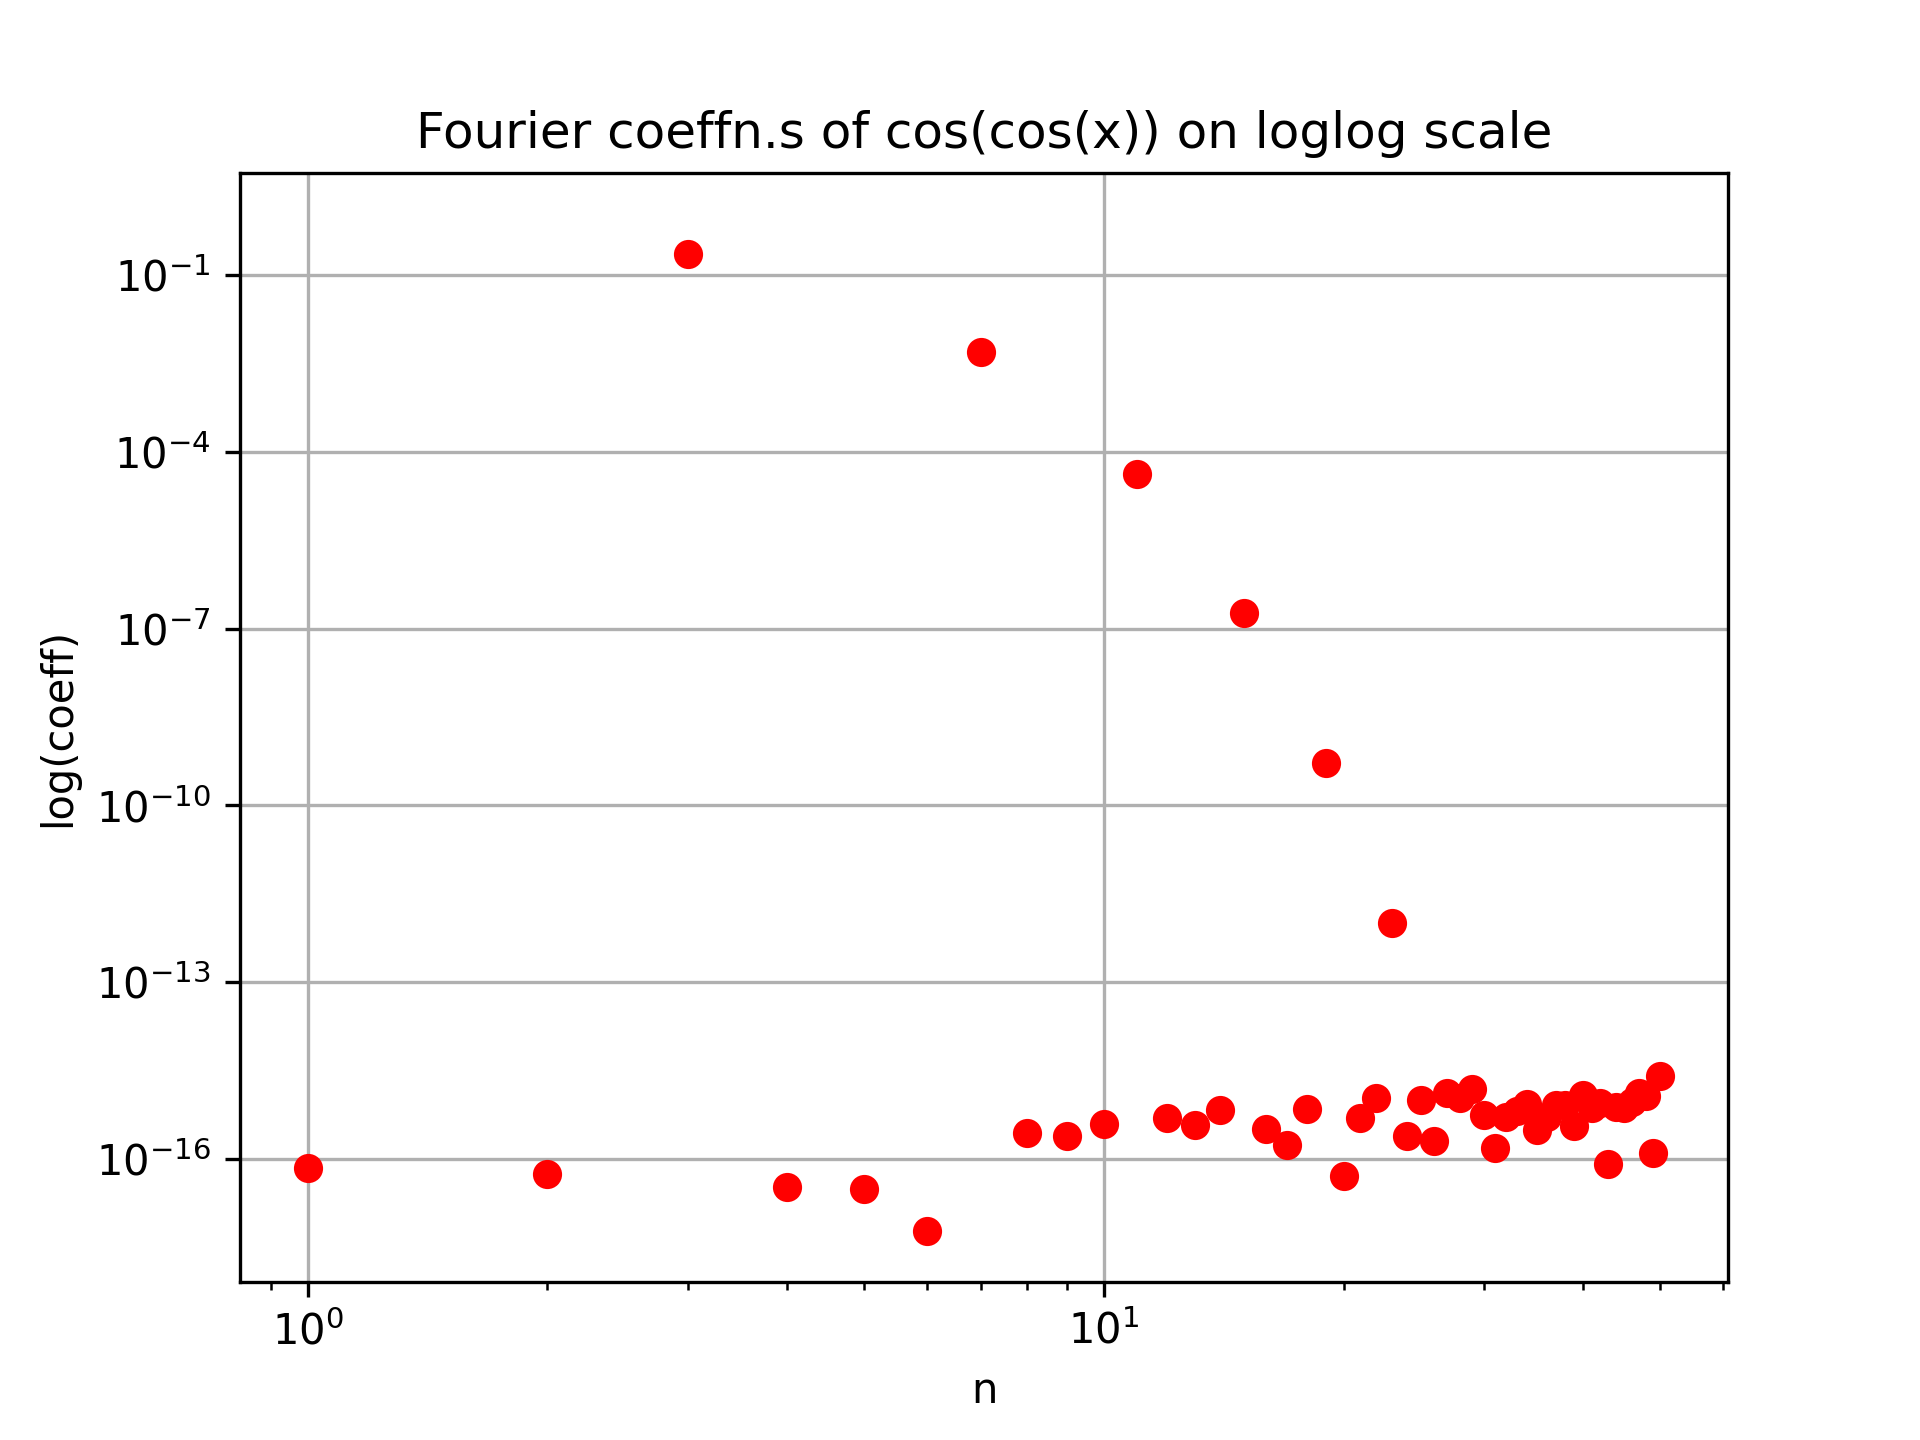
\includegraphics[scale=0.6]{assn4_plot6.png}
\caption{Figure 6}
\label{fig:plot6}
\end{figure} 

\subsection*{Question 4}
We use the least squares method to find the approximate the values of the coefficients. However , we use a small number of points(400) so the error can be quite large. If we use a larger number of points , then the error might decrease.

\subsection*{Question 5}
We solve the equation Ac=b using the lstsq method and plot the results.

\begin{figure}[!tbh]
\centering
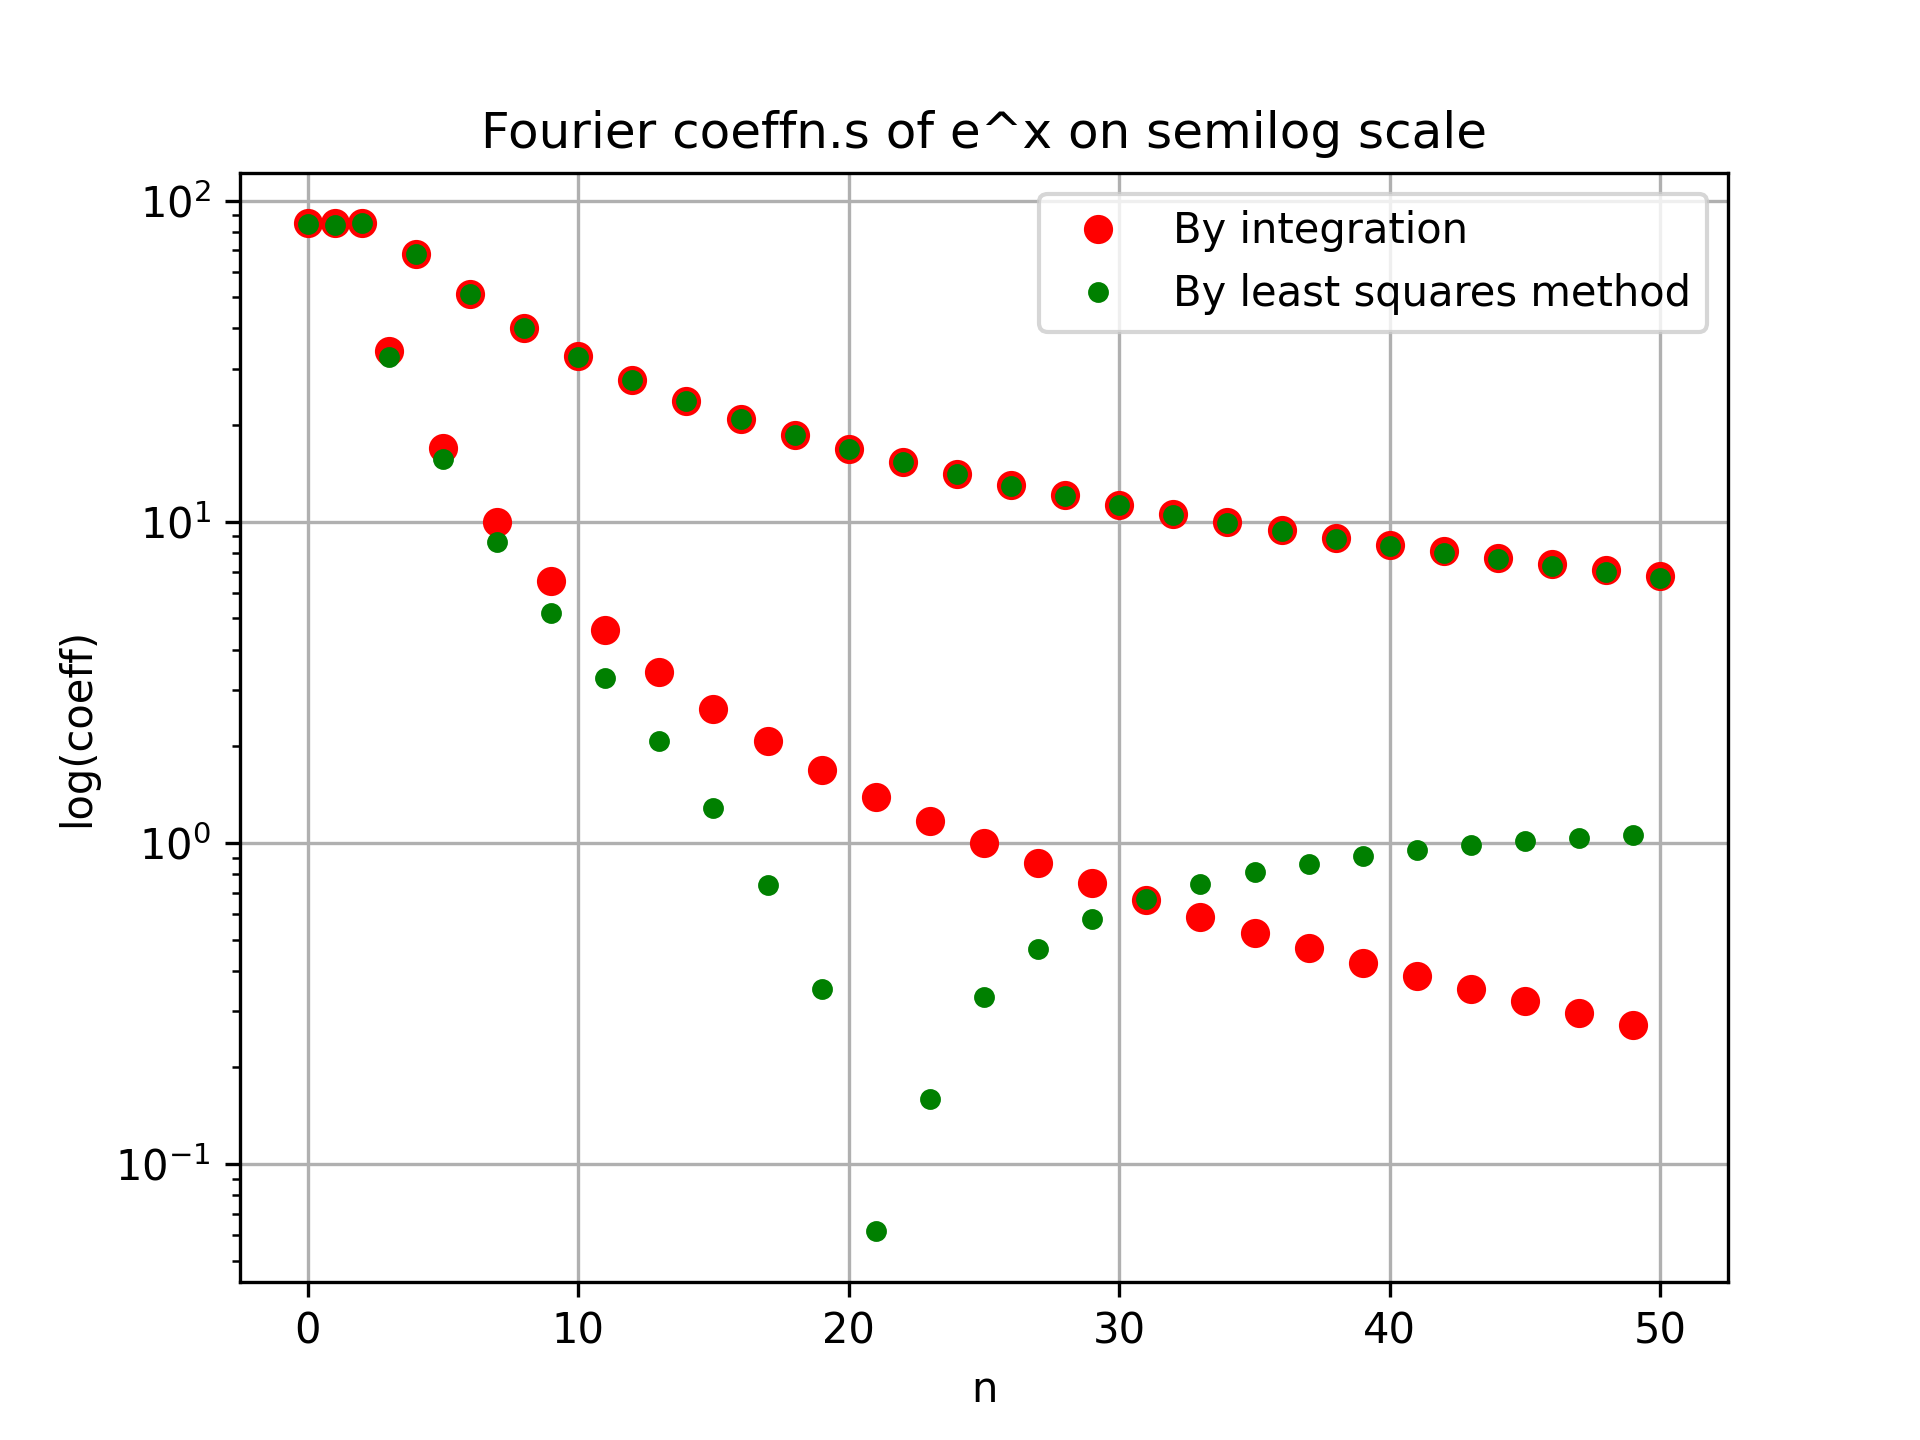
\includegraphics[scale=0.6]{assn4_plot7.png}
\caption{Figure 7}
\label{fig:plot7}
\end{figure} 

\begin{figure}[!tbh]
\centering
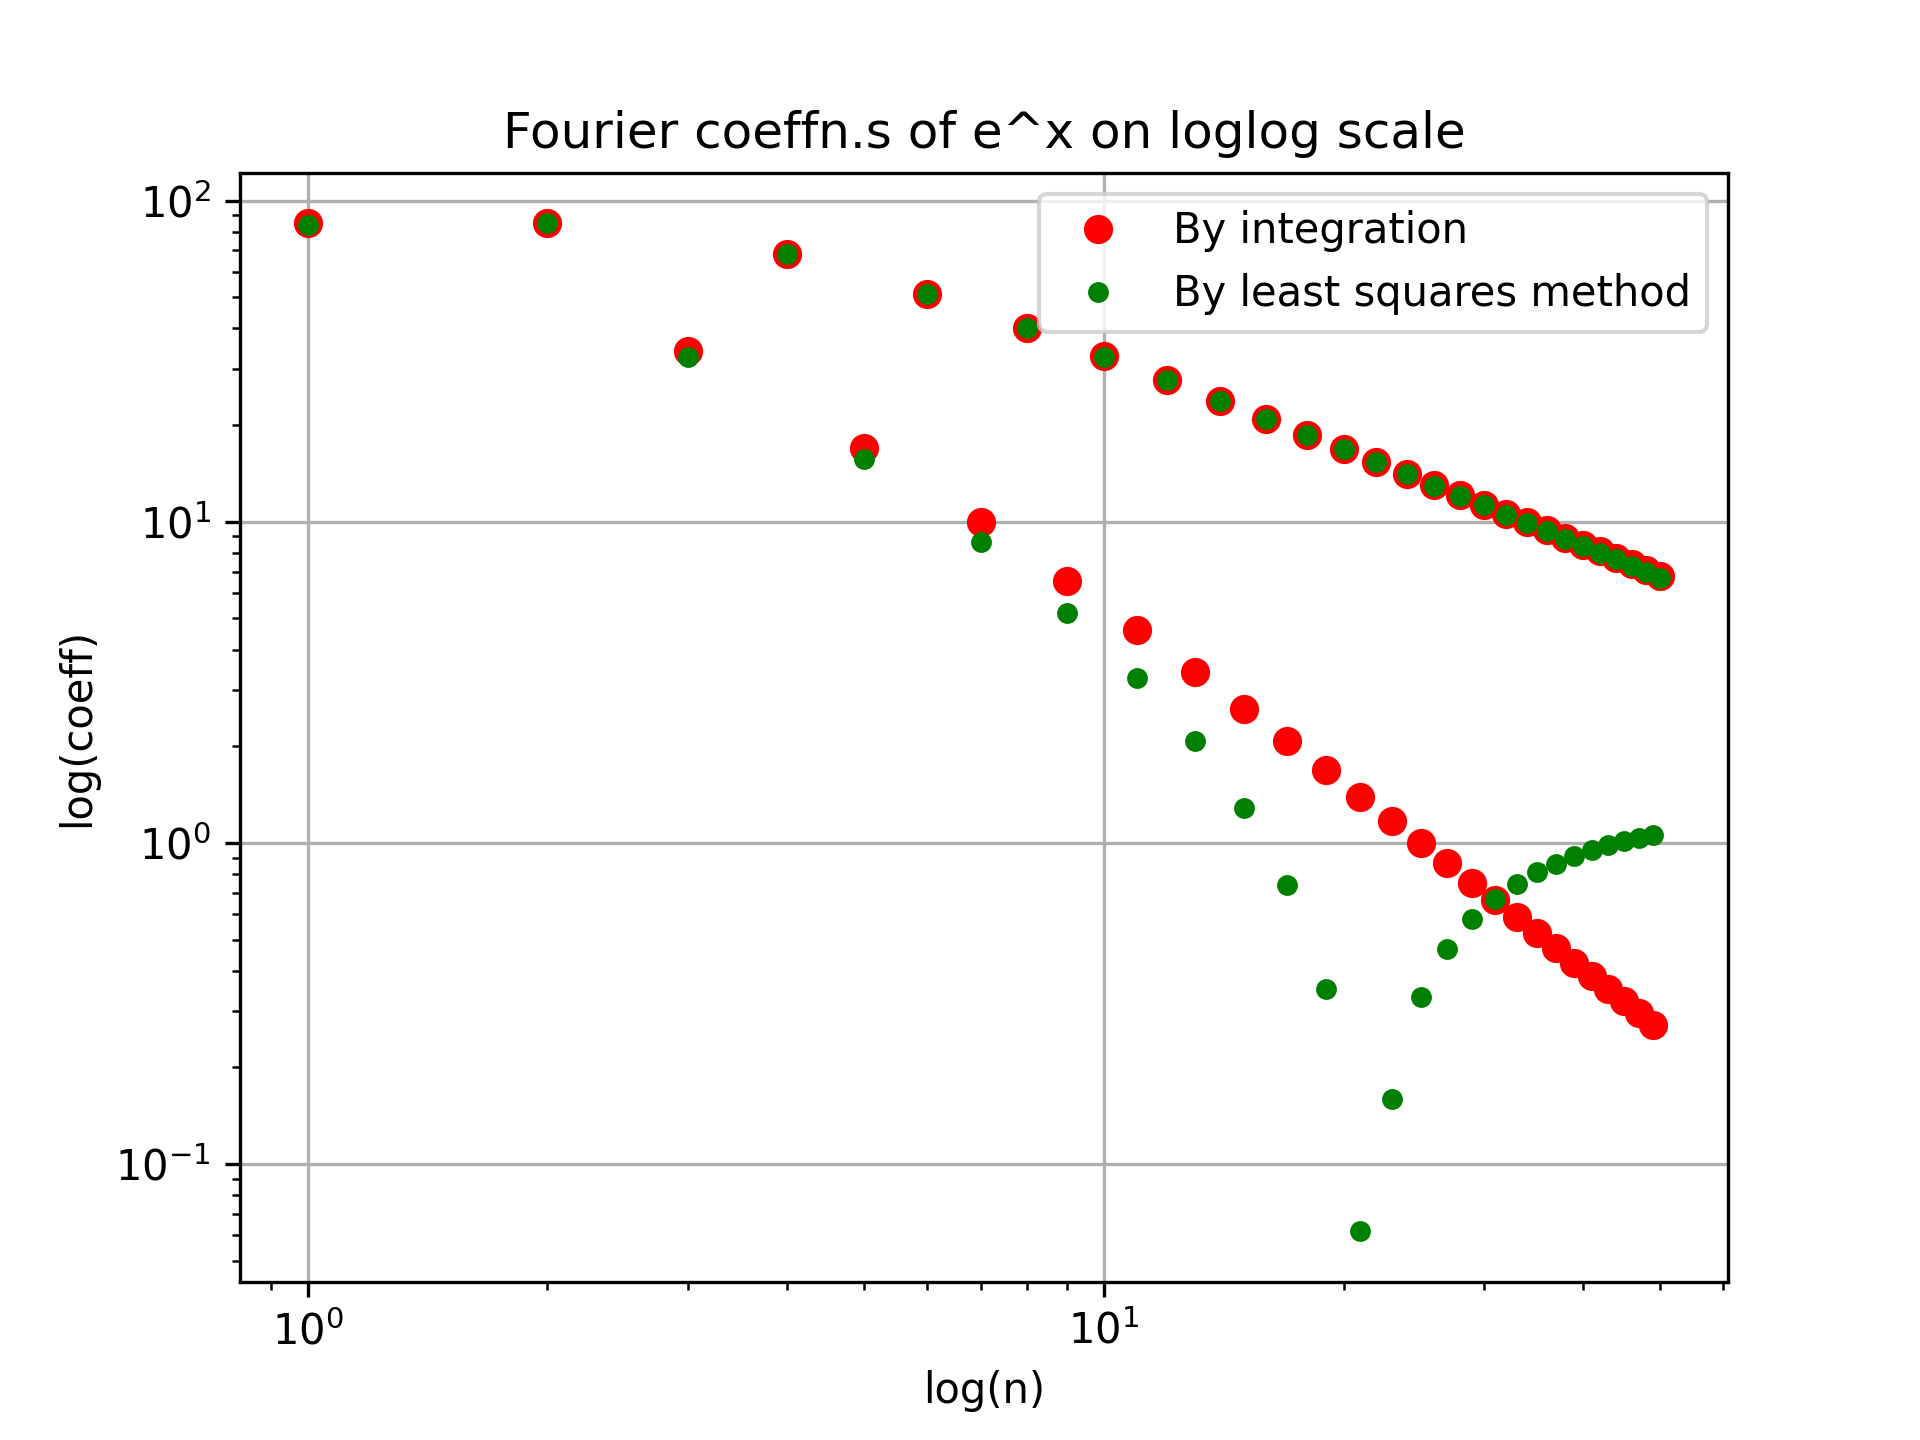
\includegraphics[scale=0.6]{assn4_plot8.png}
\caption{Figure 8}
\label{fig:plot8}
\end{figure} 

\begin{figure}[!tbh]
\centering
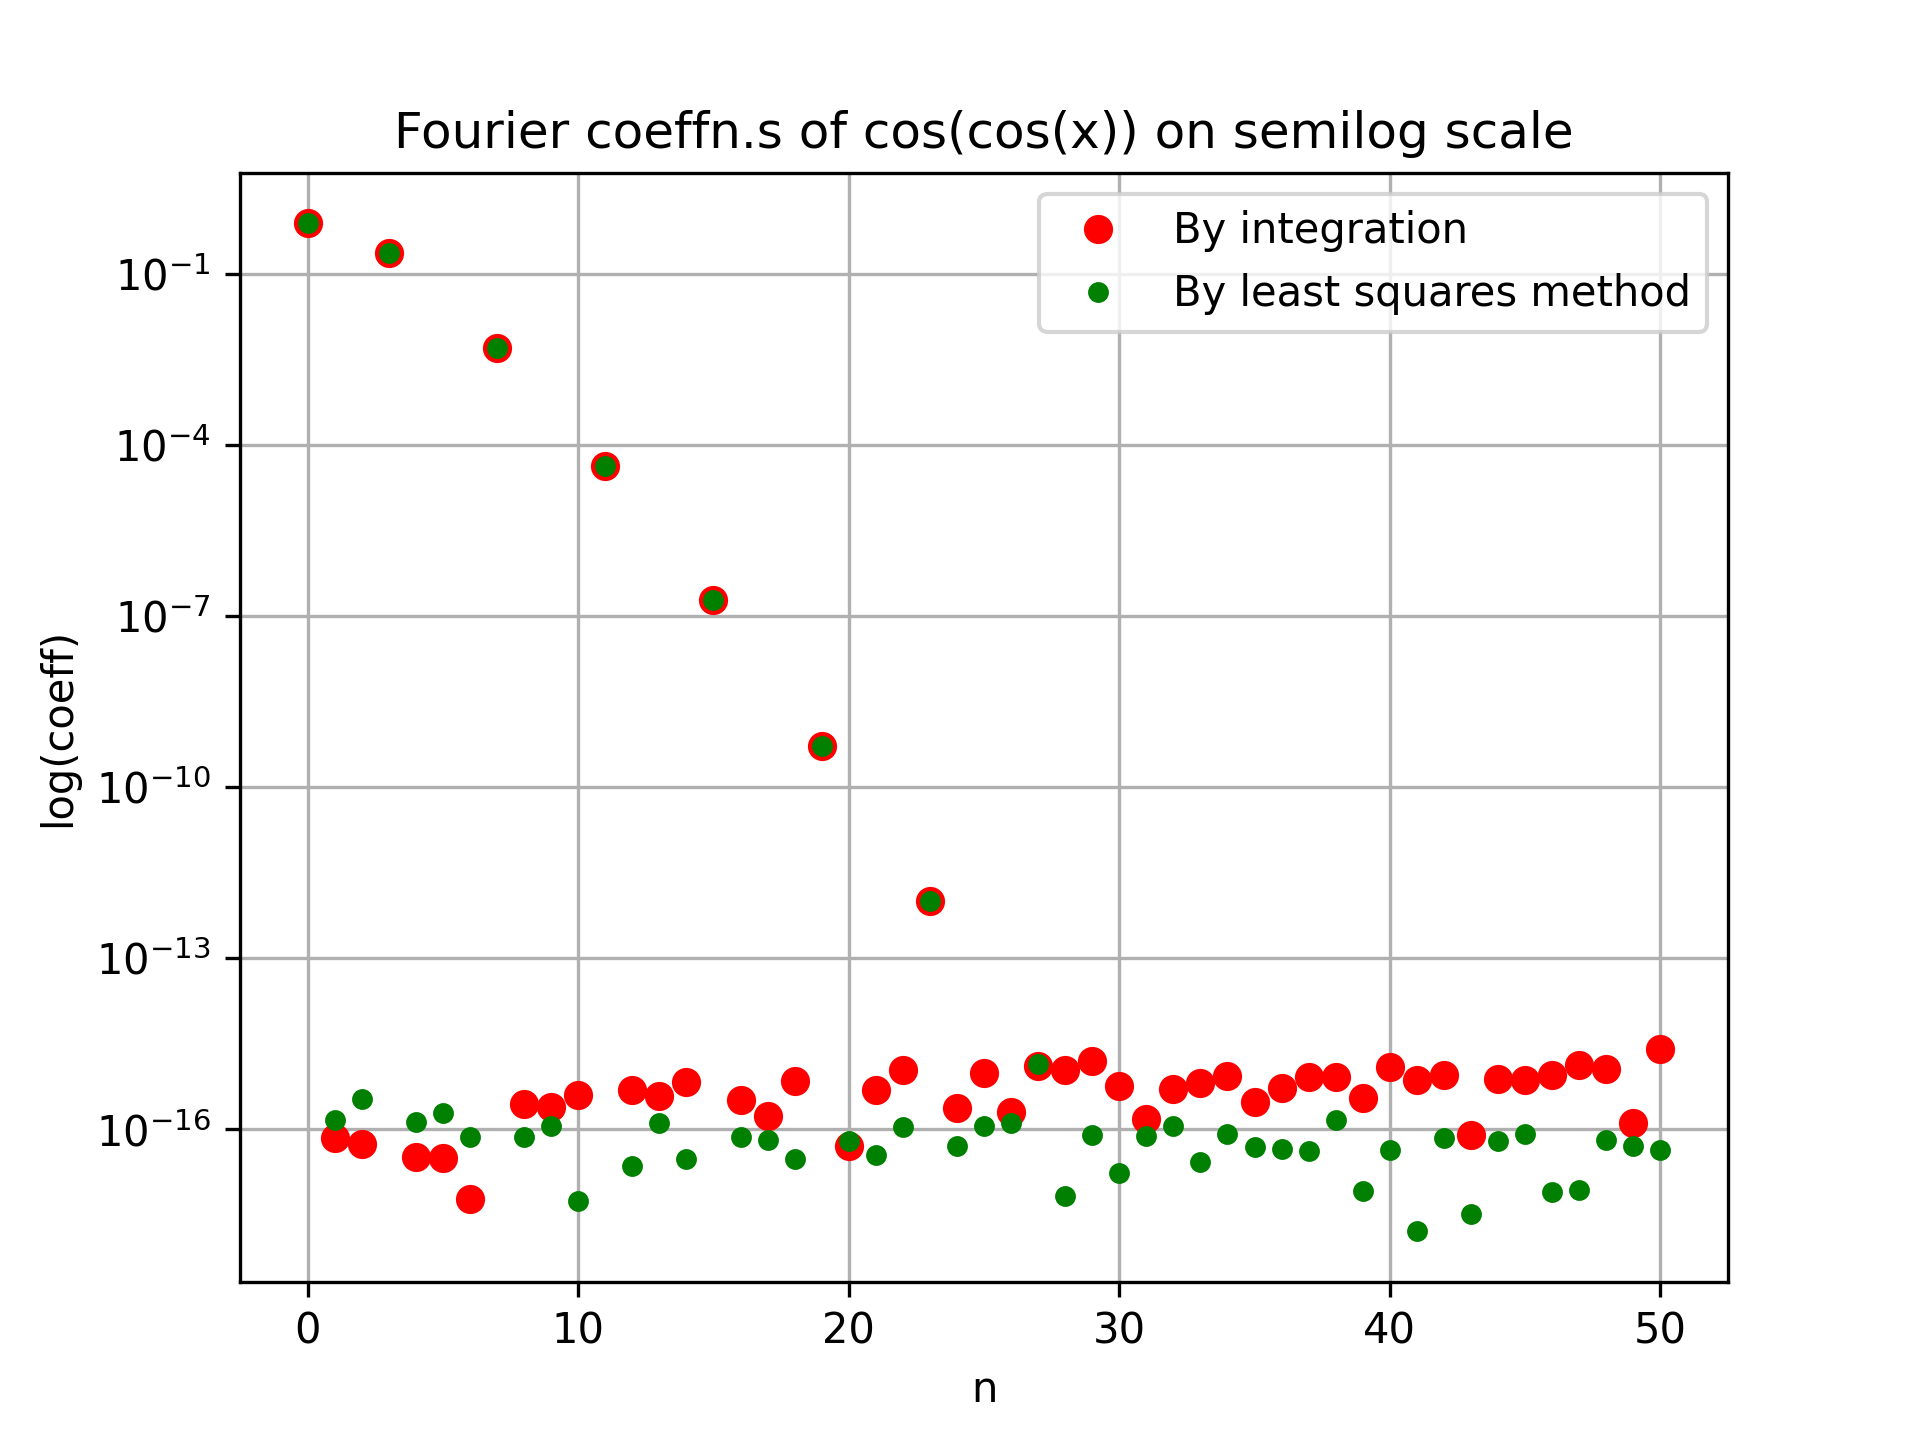
\includegraphics[scale=0.6]{assn4_plot9.png}
\caption{Figure 9}
\label{fig:plot9}
\end{figure} 

\begin{figure}[!tbh]
\centering
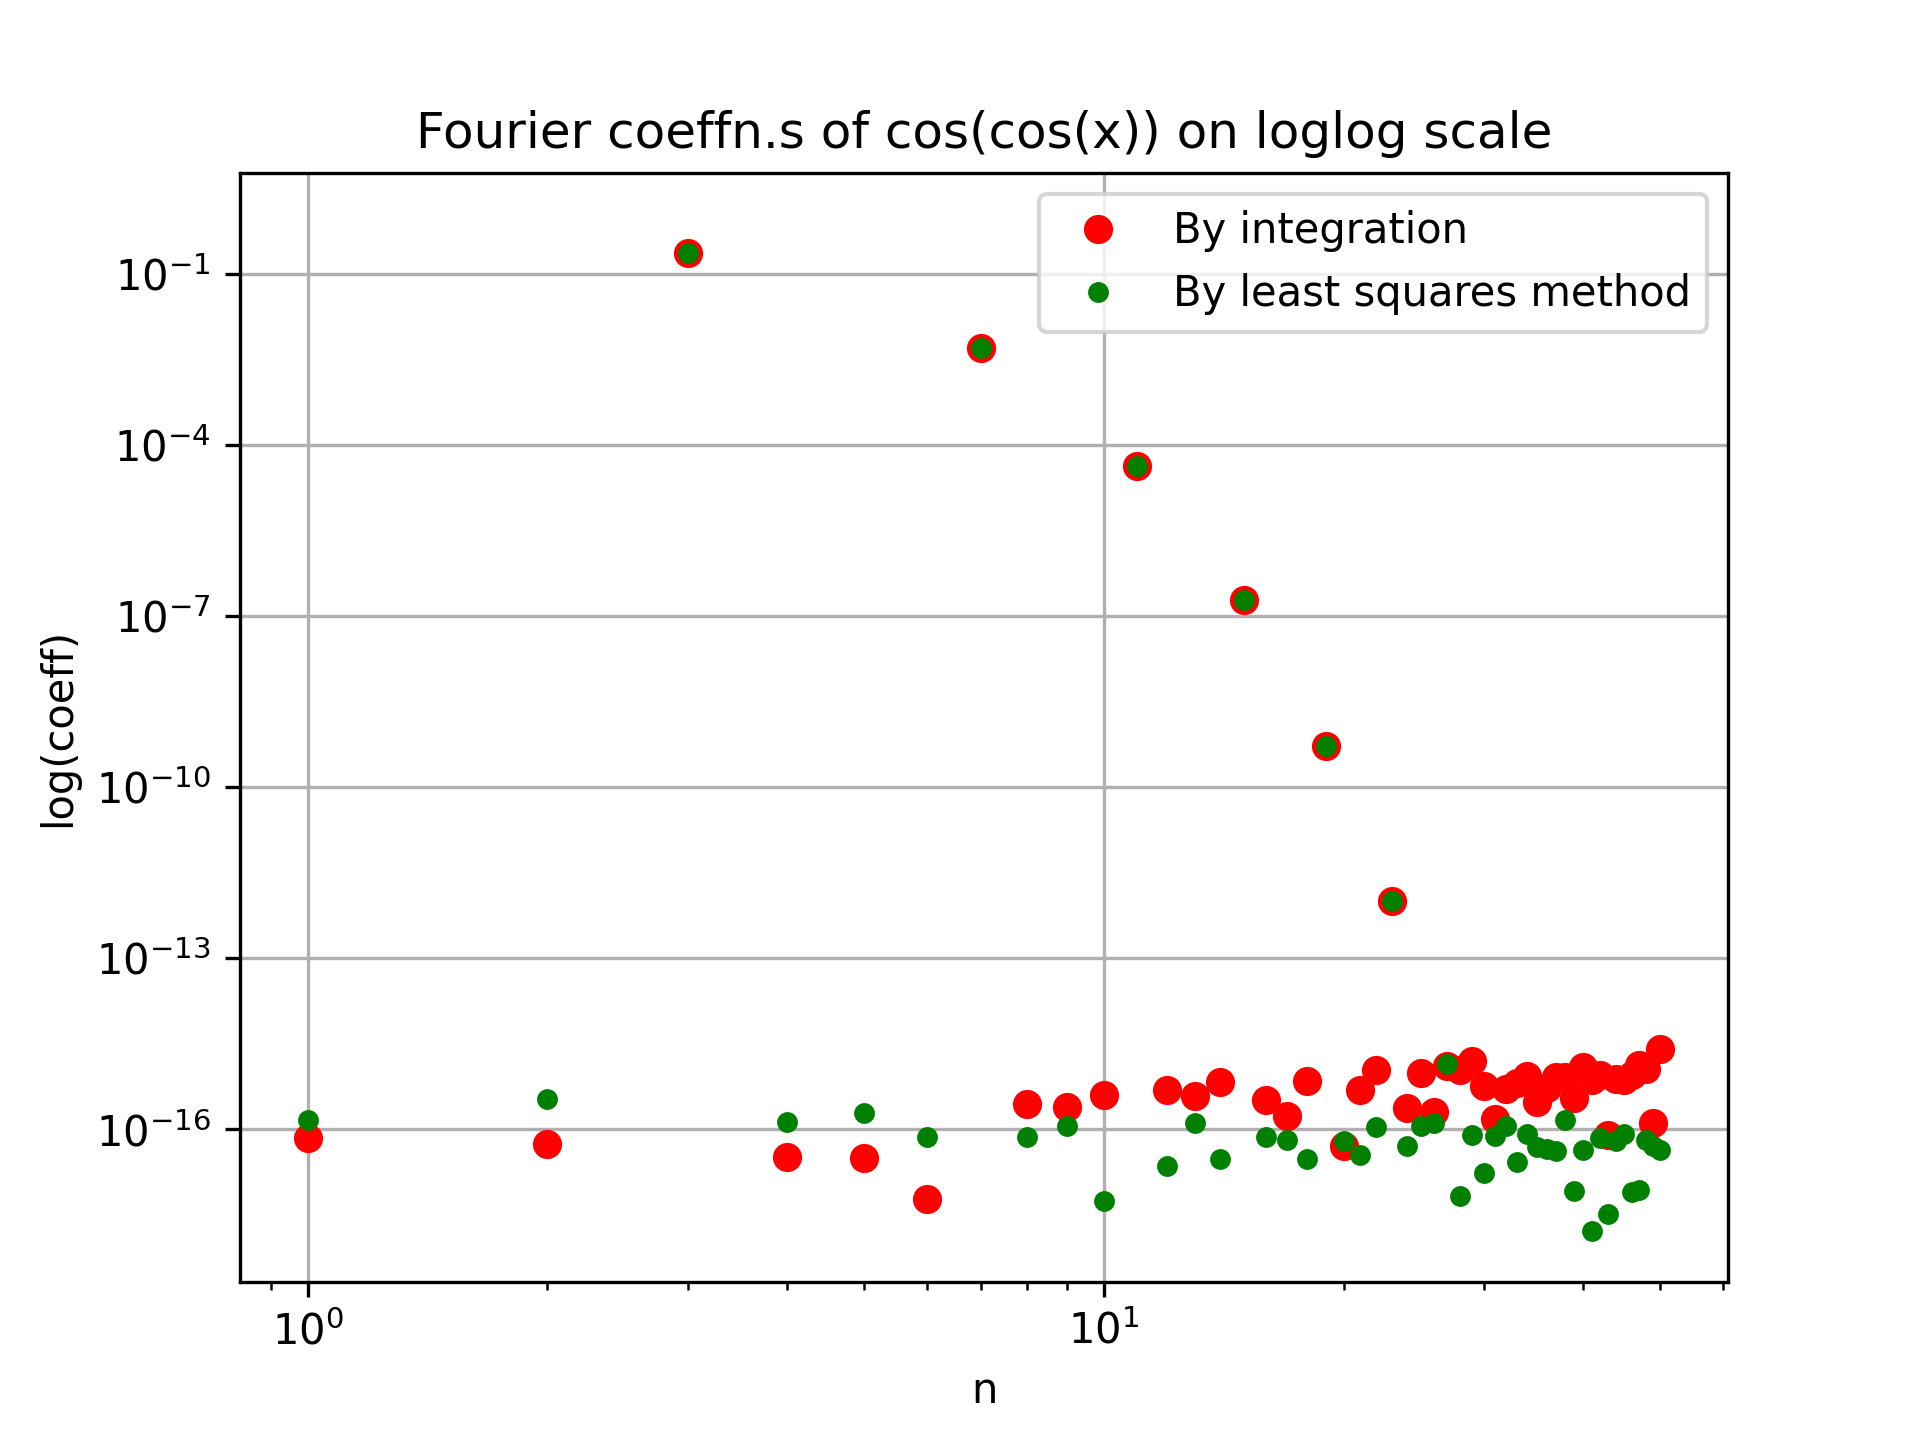
\includegraphics[scale=0.6]{assn4_plot10.png}
\caption{Figure 10}
\label{fig:plot10}
\end{figure} 

\subsection*{Question 6}

When we compare the values of the coefficients obtained by the least squares method and the direct integration method ,they should agree with each other , but we observe that there is a significant deviation of values in the $e^x$ function,probably because the number of sample points taken were very less , but the values for cos(cos(x)) are almost in agreement.

Deviation for $e^x$ =1.337
Deviation for cos(cos(x))=$2.64*10^-15$

\subsection*{Question 7}
We find the function values using the coefficients that we obtained through least squares method and we plot them.

\begin{figure}[!tbh]
\centering
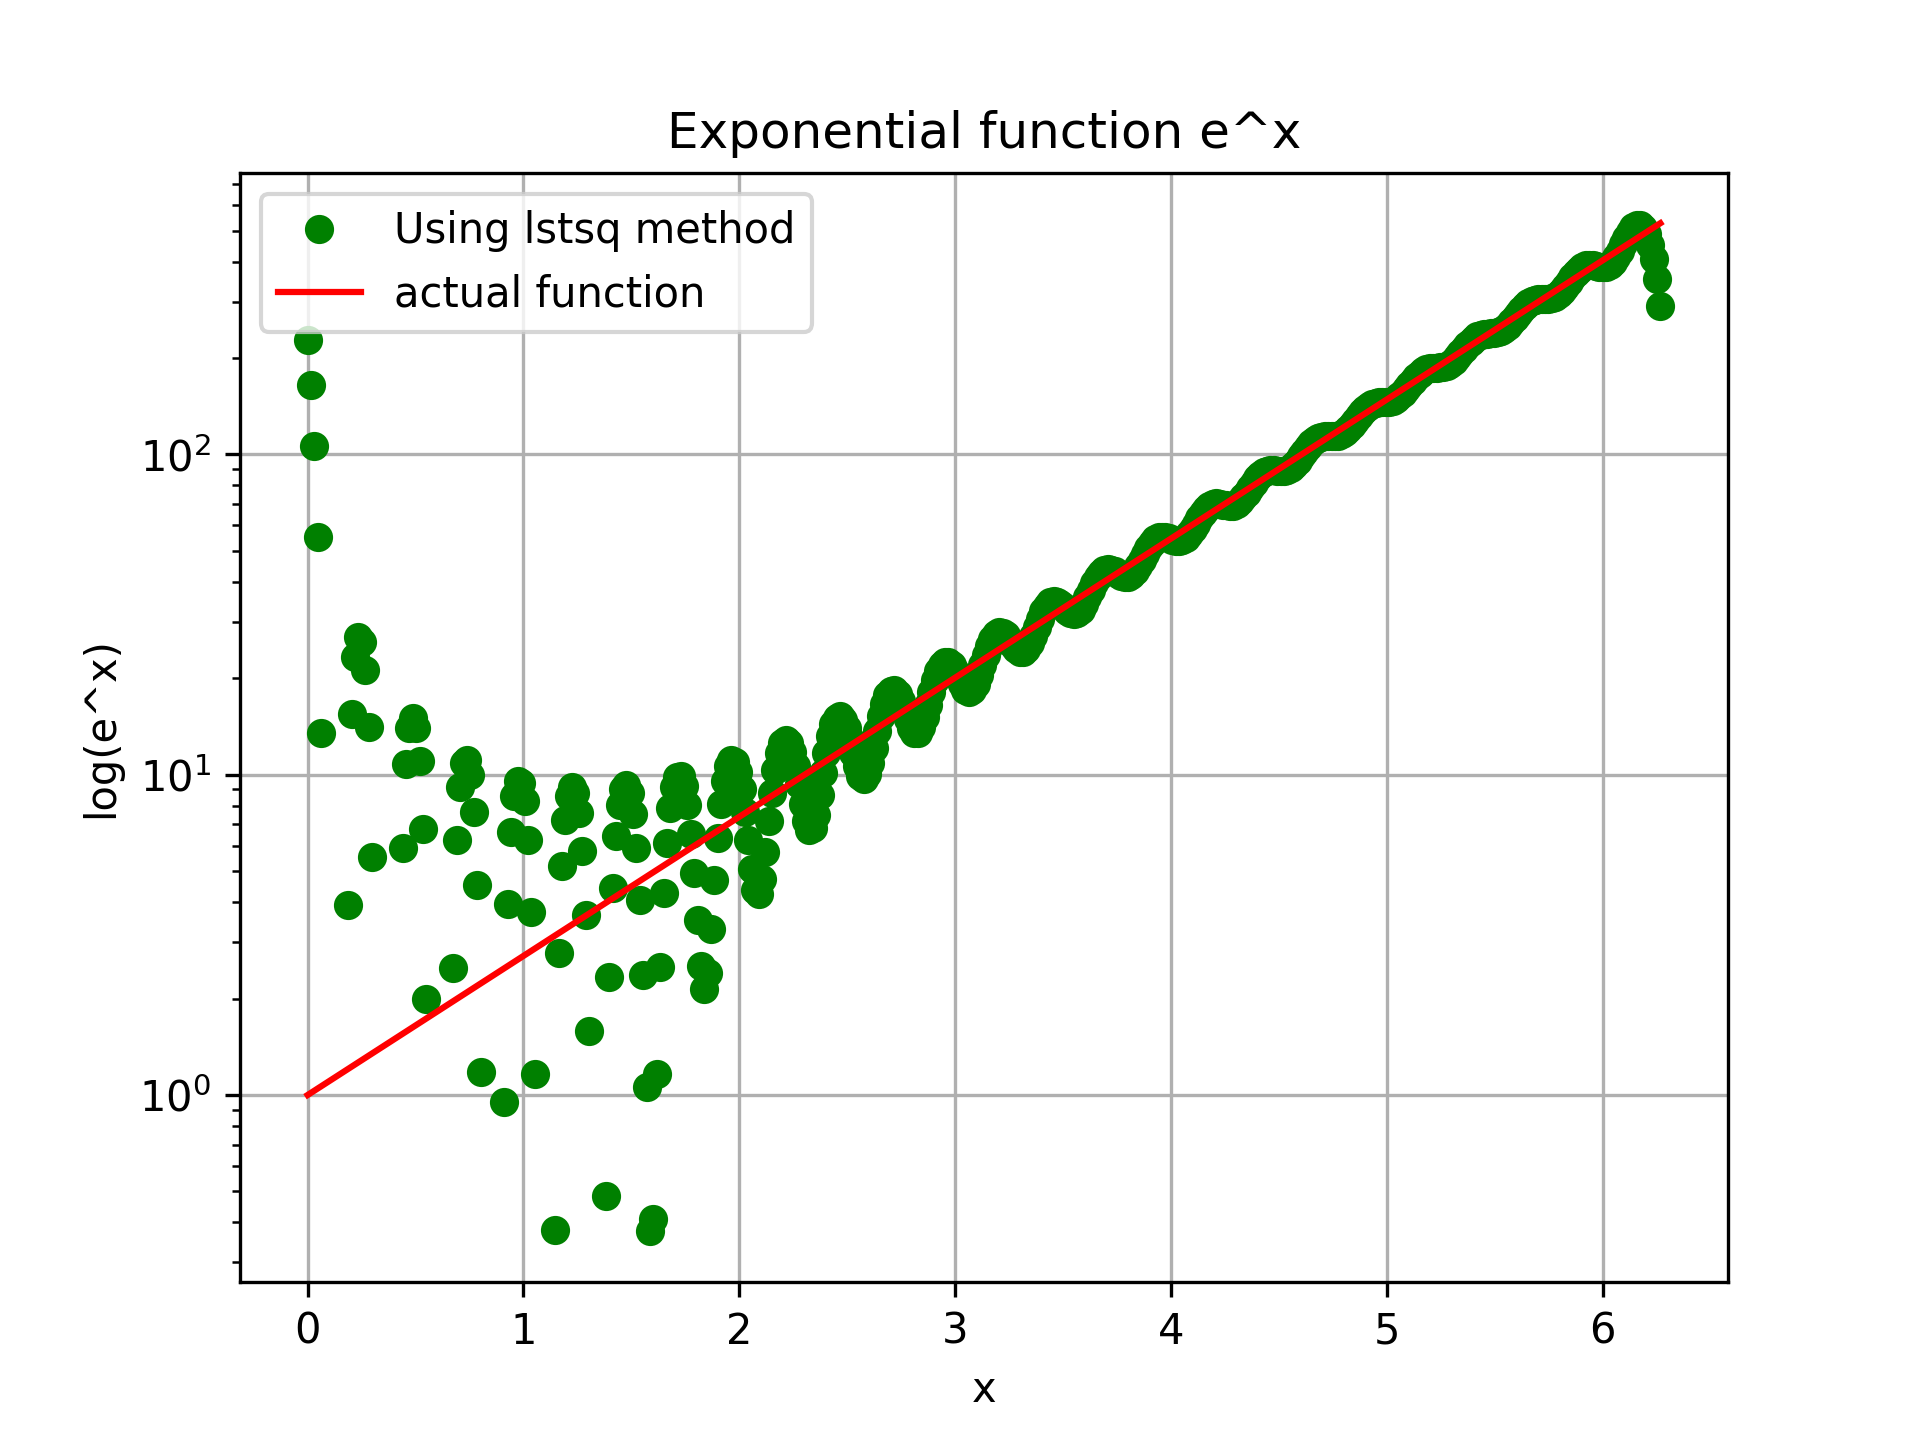
\includegraphics[scale=0.6]{assn4_plot11.png}
\caption{Figure 11}
\label{fig:plot11}
\end{figure} 

\begin{figure}[!tbh]
\centering
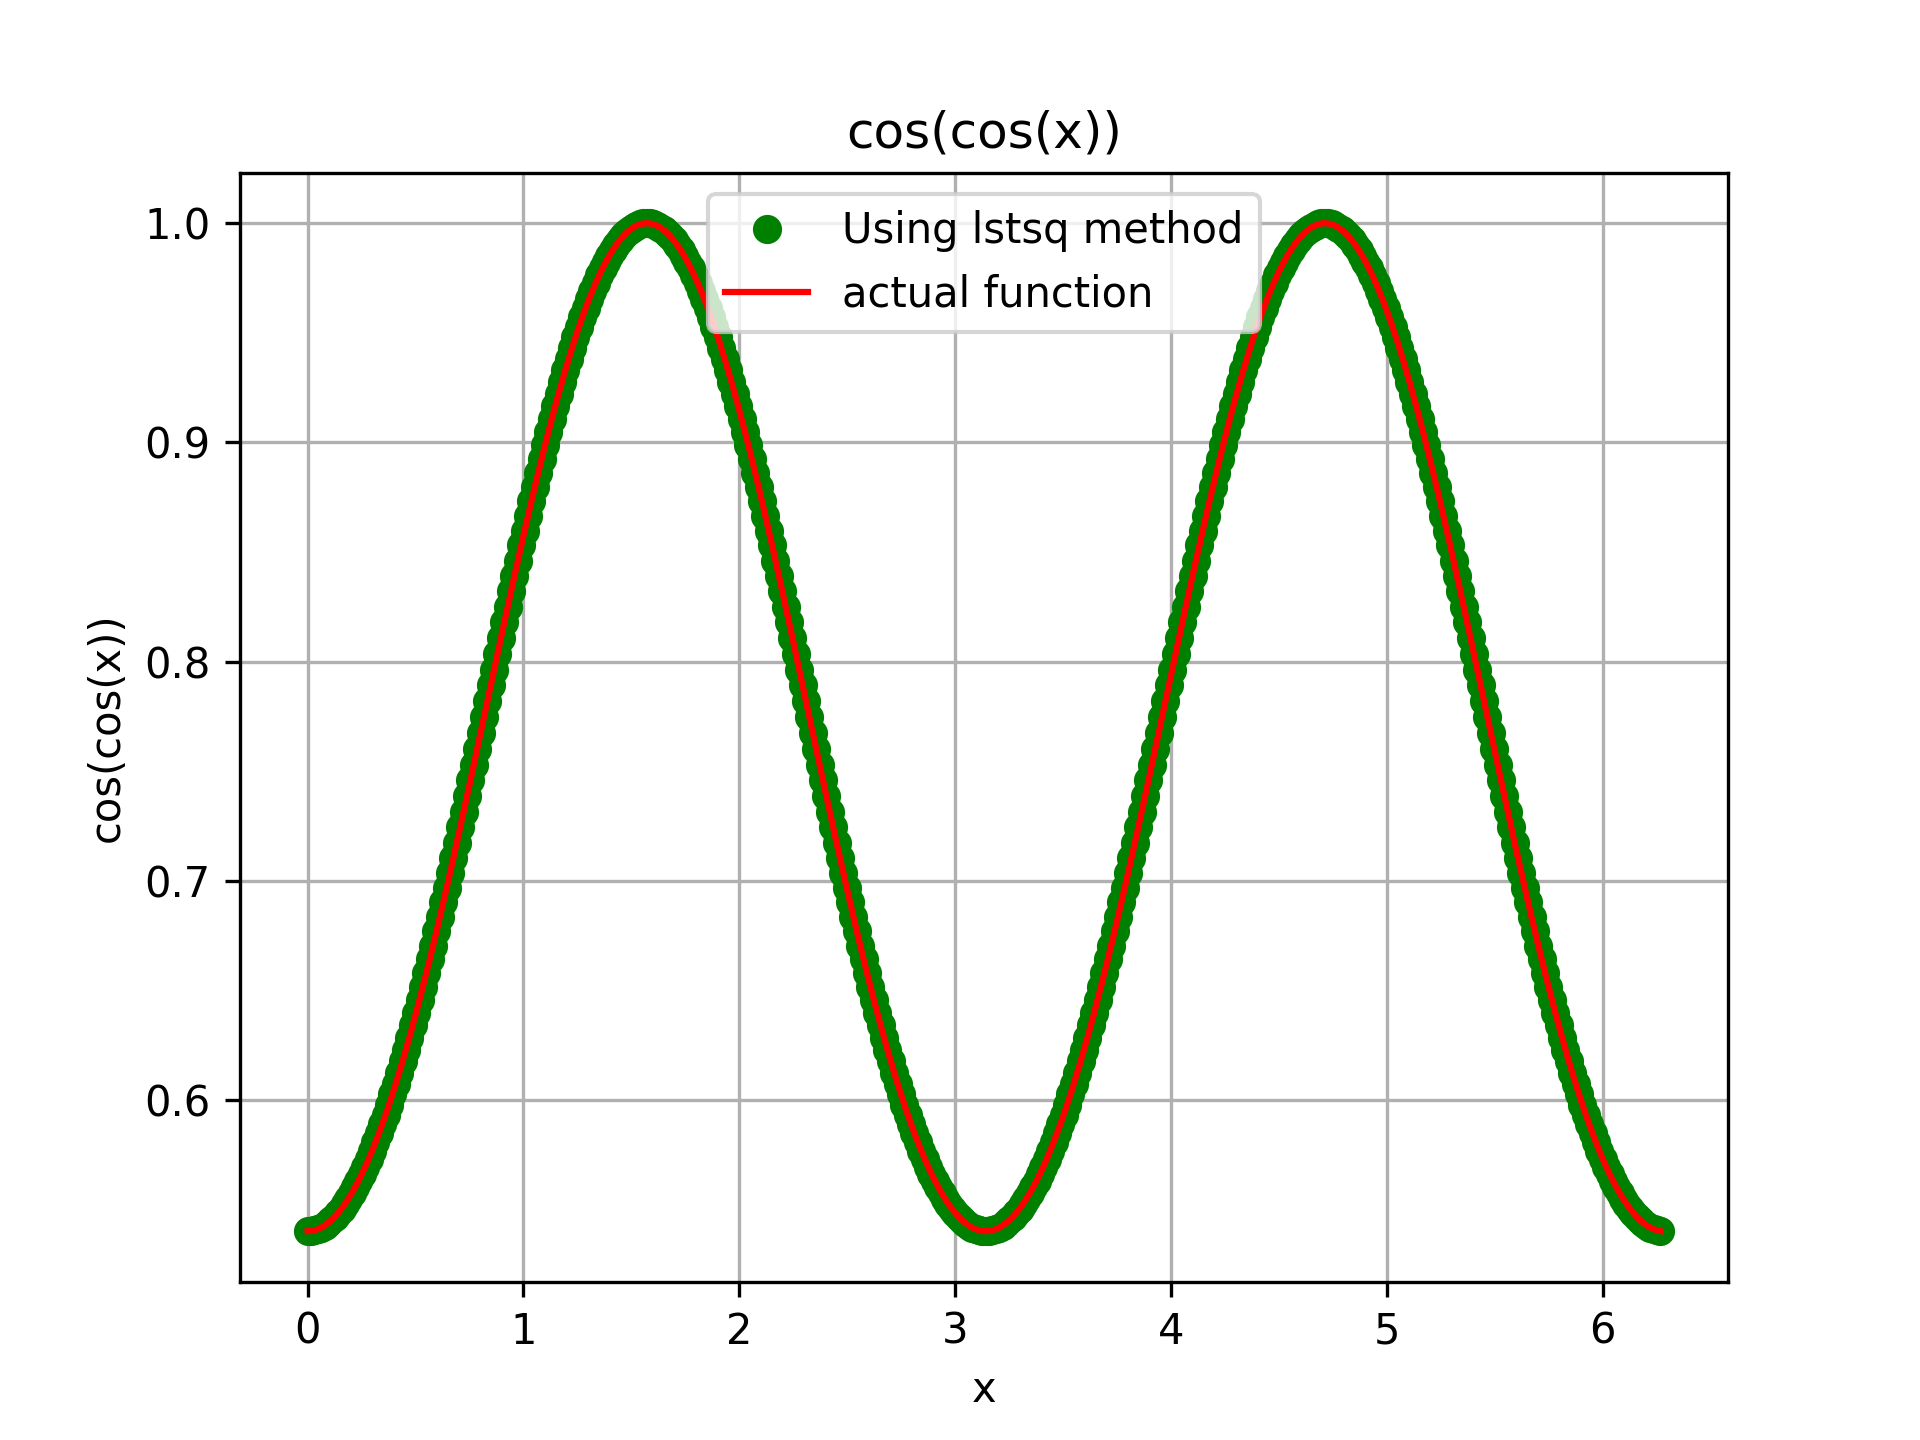
\includegraphics[scale=0.6]{assn4_plot12.png}
\caption{Figure 12}
\label{fig:plot12}
\end{figure} 

\section*{Conclusion}
We have seen two ways of calculating fourier coefficients, by direct integration and by the least squares method. We have seen that the error in the coefficients when calculated by using lstsq method is not very large , especially when we use a large number of sample points. Hence , it is safe to use the least squares method for these functions and reduce the computation complexity.

\end{document}
